Libraries, structured and curated collections of informational resources, play a key role in preserving the collective memory of the human civilisation and its heritage. The resources they store take various structural (manuscripts, media, articles) and semantic (historic content, research, literature) forms and are made available to either the general public, or more fine-grained user groups.

With the advent of the world wide web (WWW) in the late 20th century, libraries were among the first applications of the new online technologies, giving rise to \emph{digital} libraries. It can be argued that the WWW as a whole represents in itself a library; still, discrete instances can maintain the structural and semantic differentiation mentioned previously and can better target various user groups, catering to their specific needs.

The evolution of digital libraries in the past 30 years was greatly influenced by the evolution of scholarship and scientific research. First, funding for such activities has greatly increased, as presented in Fig. \ref{fig:fundig} and, as a direct result, the number of outputs, such as monographs, journal articles or theses, has increased (see Fig. \ref{fig:nopublications}). This impacted digital libraries which now need to be able to manage a larger influx of new content, while ensuring its proper dissemination across stakeholders. 
\begin{figure}[ht!]
\centering
\begin{subfigure}{0.9\textwidth}
  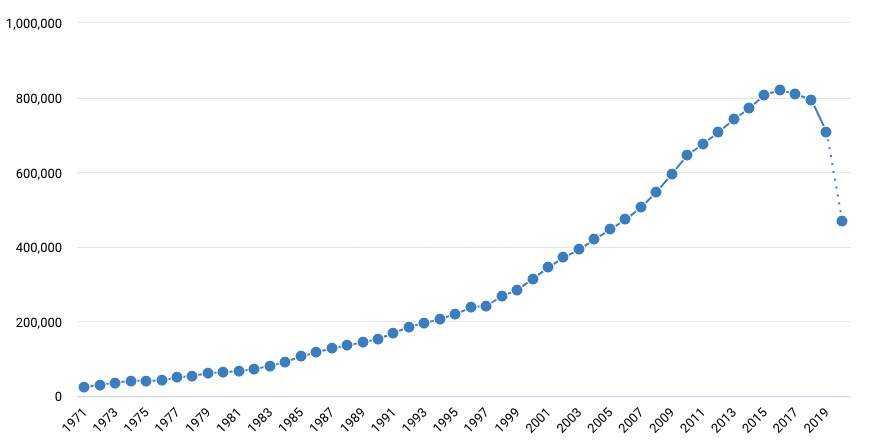
\includegraphics[width=1\linewidth]{no_grants.png}  
  \caption{Evolution of number of research grants since 1971. Data since 2018 is incomplete.}
  \label{subfig:grants}
\end{subfigure}
\begin{subfigure}{0.9\textwidth}
  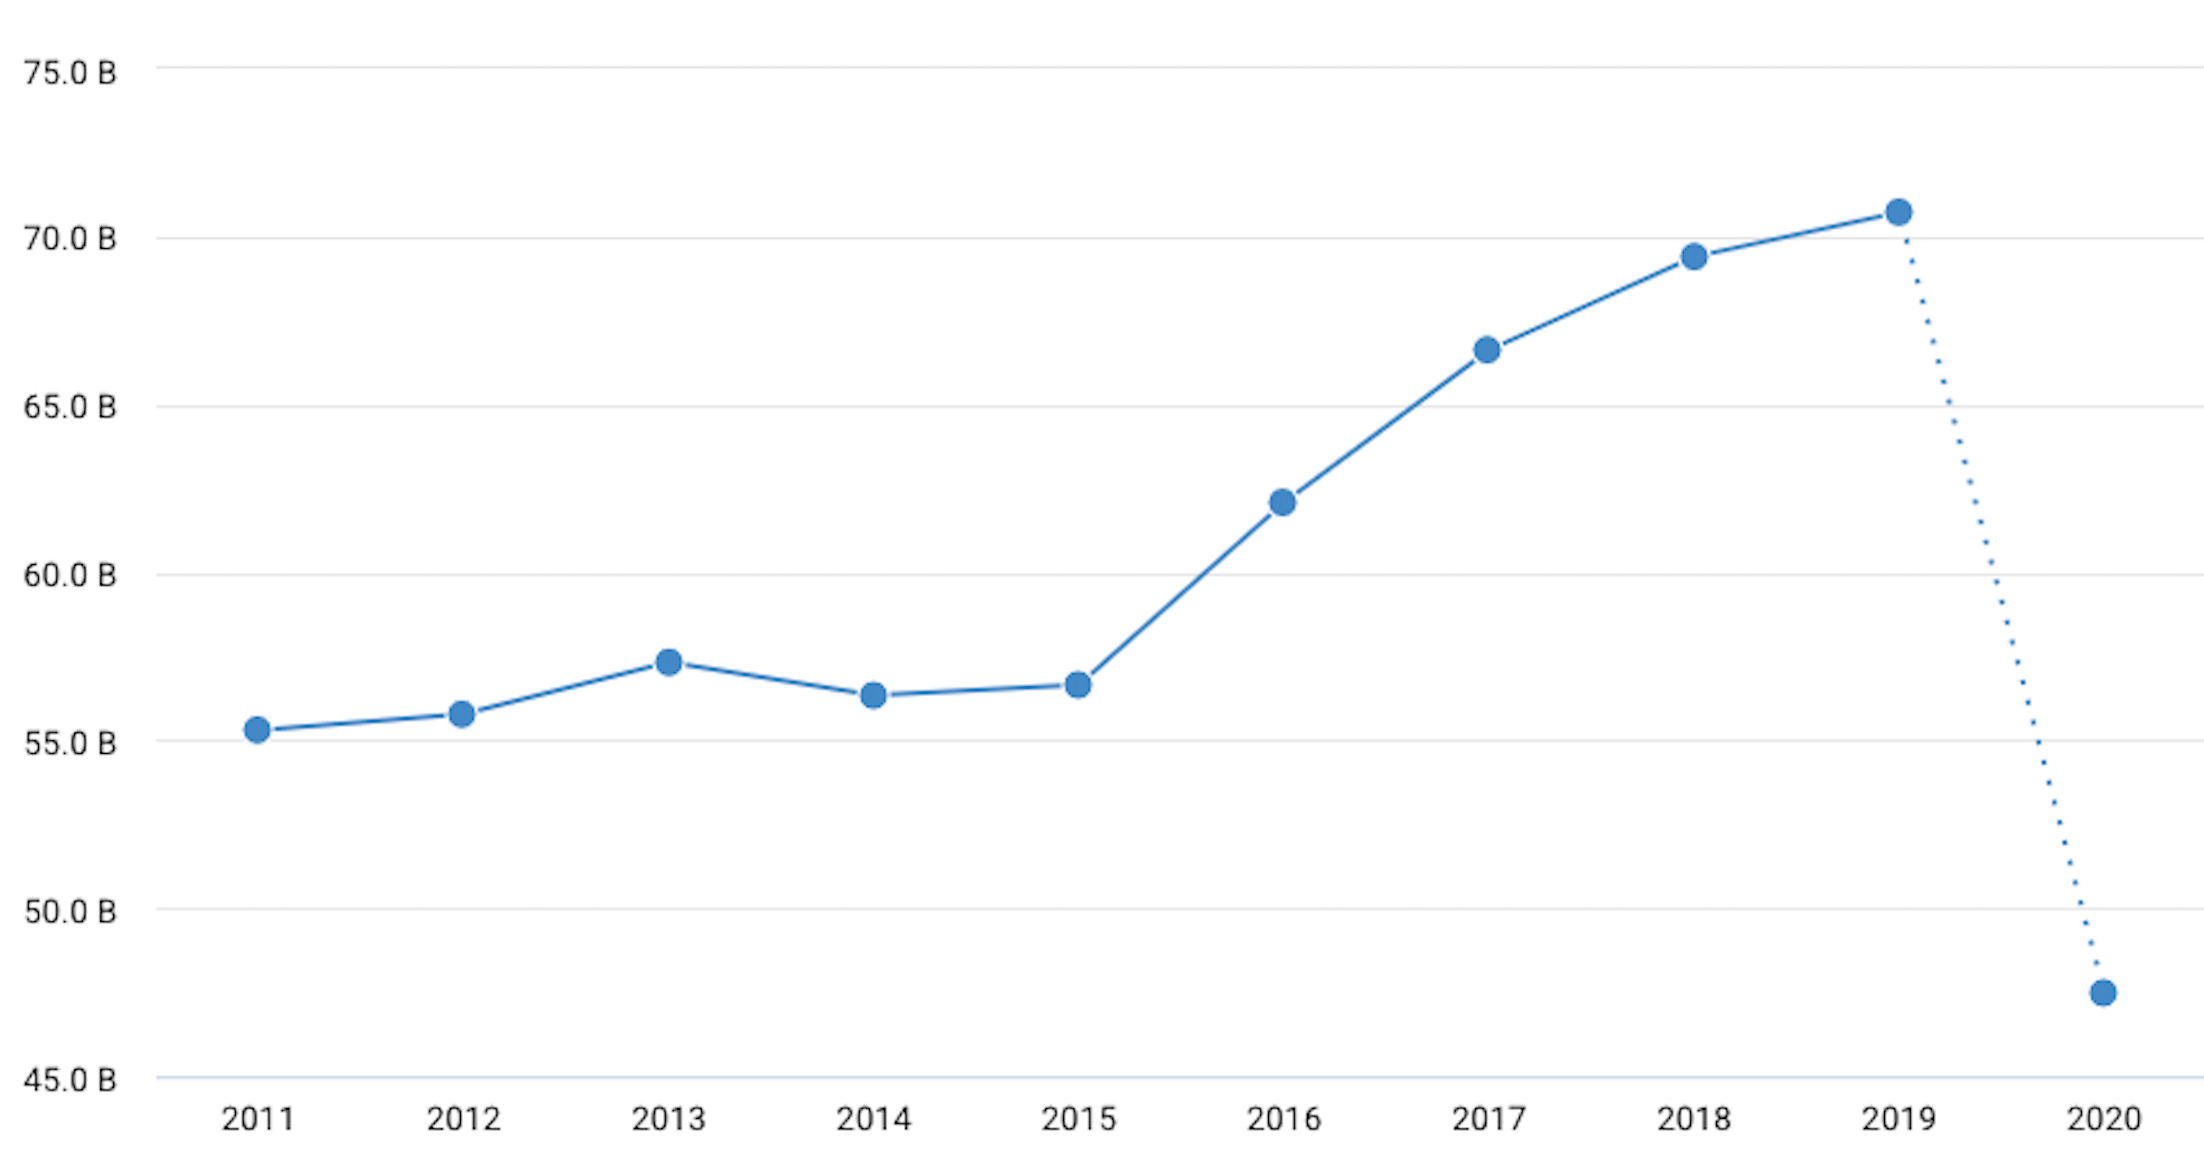
\includegraphics[width=1\linewidth]{funding.png}  
  \caption{Evolution of total amount of research grants since 2011, in pounds sterling. Data for 2020 is incomplete.}
  \label{subfig:grantstotal}
\end{subfigure}
\caption{Evolution of research funding, source \url{https://app.dimensions.ai}}
\label{fig:fundig}
\end{figure}

\begin{figure}[ht!]
\centering
  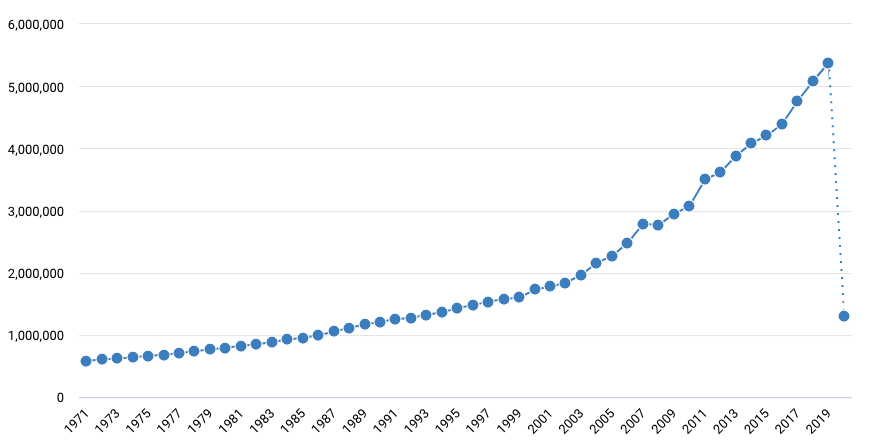
\includegraphics[width=1\linewidth]{publications.png}  
  \caption{Evolution of number of research publications, data since 2019 is incomplete.}
  \label{fig:nopublications}
\end{figure}

Second, a number of significant events in the area of research and scholarly communications have taken place; two of these of of interest.

The \emph{\gls{oa}} reforms came to prominence along with digital libraries; as the medium for disseminating research switched from physical (paper journals or monographs) to digital, researchers questioned the suitability of the traditional business plans of publishers (e.g., Springer Nature or Elsevier), which could no longer fully justify the costs inquired for typesetting and printing, among others. \gls{oa} is one proposed way of resolving this, its aim being to shift the costs of publishing from being supported by consumers to being supported by producers (i.e., researchers wishing to disseminate their work, or, most often, their funders). \gls{oa} can be practically implemented in various forms, but of interest here is the so-called \emph{green} \gls{oa}; in this model, researchers are allowed to self-publish a version of, for example, their peer-reviewed journal article which does not includes the publishers typesetting or copy-editing. A common platform for this is the digital library managed by the researcher's institution.

The \emph{reproducibility crisis} is a phenomenon generated by a number of research studies that failed to \emph{replicate}, other researchers not being able to verify the claims of the original authors by repeating similar experiments. An infamous such example is a paper\footnote{Wakefield et. al. (1998) \emph{RETRACTED: Ileal-lymphoid-nodular hyperplasia, non-specific colitis, and pervasive developmental disorder in children}} published in 1998 in The Lancet which linked the measles, mumps and rubella vaccine to colitis and autism spectrum disorders in children. The paper was lately retracted, due to evidence of fraud, conflicts of interest and manipulation of data. The literature currently documents multiple instances of studies that exhibit reproducibility or replication\footnote{It is widely accepted that \emph{reproducibility} is the act of reaching original research result by using the same research materials (data, software, instruments), while \emph{replicability} uses different inputs (e.g., a new set of patients for a clinical study) in order to reach similar results\cite{patil}.} issues, due to, among others, technical, methodology or workflow faults (see, for example \cite{eklund,seekblastn}).

As a result of this crisis, the world of research focused in latest years on ensuring that published scientific result are accompanied by all the required artefacts (e.g., data, software, protocols) necessary to allow other researchers to fully verify the claims of the original authors. This move was also formalised by both research funding bodies\cite{h2020,nih}\footnote{It is important to note that at least the mentioned funding bodies also needed to ensure that all research funded from public income becomes publicly available; this is also linked with the \gls{oa} policies.} and publishers\cite{scidat,elsdat}, such that good practices are enforced across the whole scientific community.

For digital research libraries this meant, above everything, adapting to the new types of outputs; data sets or scientific software present new challenges, due to their structural and semantic particularities. Moreover, libraries need to ensure that all outputs generated by a scientific study are presented in a coherent and consolidated manner, in order to facilitate reproducibility.

This work provides a description of the evolution of digital libraries, in light of the two challenges mentioned above, showing how this type of applications have overcome them by developing new features and workflows. Furthermore it introduces a number of novel solutions to existing issues, by employing state-of-art technologies and software engineering practices. A note here is that librarians need to adapt to the new realities, by including software-assisted workflows and tools in their craft\footnote{As an example, see the Software Carpentry project at \url{https://software-carpentry.org/blog/2015/05/coding-for-librarians.html}.}.

Across the work the term \emph{repository} will be used; this comes from the widespread term \gls{ir}, which defines an archive of intellectual outputs of a research institution, most often a university. \glspl{ir} are a subset of digital libraries, as the latter could also hold content which is not scientific in nature. For clarity, a distinction between \emph{institutional} repositories (holding scientific \emph{literature}), \emph{data} repositories, and \emph{research} repositories (holding any type of outputs) is employed, this being useful for understanding the evolution of this type of platform.